\documentclass[11pt]{article}

\usepackage[left=1in, right=1in, top=1in, bottom=1in, paperwidth=8.5in, paperheight=60in]{geometry} % Adjust 'paperheight' as needed

\usepackage{graphics,epsfig,graphicx,float,subfigure,color}
\usepackage{algorithm,algorithmic}
\usepackage{amsmath,amssymb,amsbsy,amsfonts,amsthm}
\usepackage[small,bf,up]{caption}


\usepackage{soul}
\usepackage{comment}
\usepackage{url}
\usepackage{boxedminipage}
\usepackage[sf,bf,small]{titlesec}
\usepackage[textsize=footnotesize]{todonotes}
\usepackage[plainpages=false, colorlinks=true,
   citecolor=blue, filecolor=blue, linkcolor=blue,
   urlcolor=blue]{hyperref}

\usepackage{amsmath}

\include{ogmacros}

\newcommand{\bdm}{\begin{displaymath}}
\newcommand{\edm}{\end{displaymath}}

\newcommand{\ben}{\begin{enumerate}}
\newcommand{\een}{\end{enumerate}}

\newcommand{\p}{\partial}
\newcommand{\bs}{\boldsymbol}

\usepackage{amssymb}

%$\mathbb{R}$
\newcommand{\zapspace}{\topsep=0pt\partopsep=0pt\itemsep=0pt\parskip=0pt}

\parskip 1ex

\parindent 0ex
\begin{document}
\pagestyle{empty}

\begin{center}
{\large {\bf MATH 140: Mathematical Methods for Optimization}}\\
{\bf Assignment 7---Spring 2024}\\
{\bf Due April 4th, 2024} \\
{\textcolor{red}{\bf By:Ronald Nap}}

\end{center}

\begin{enumerate}

\item ({\bf 20 points}, the trust-region method)
  \begin{enumerate}
  \item Implement the trust-region method in matlab or python
    (algorithms 1 and 2 listed on page 2).

    \begin{figure}[H]
    \centering
    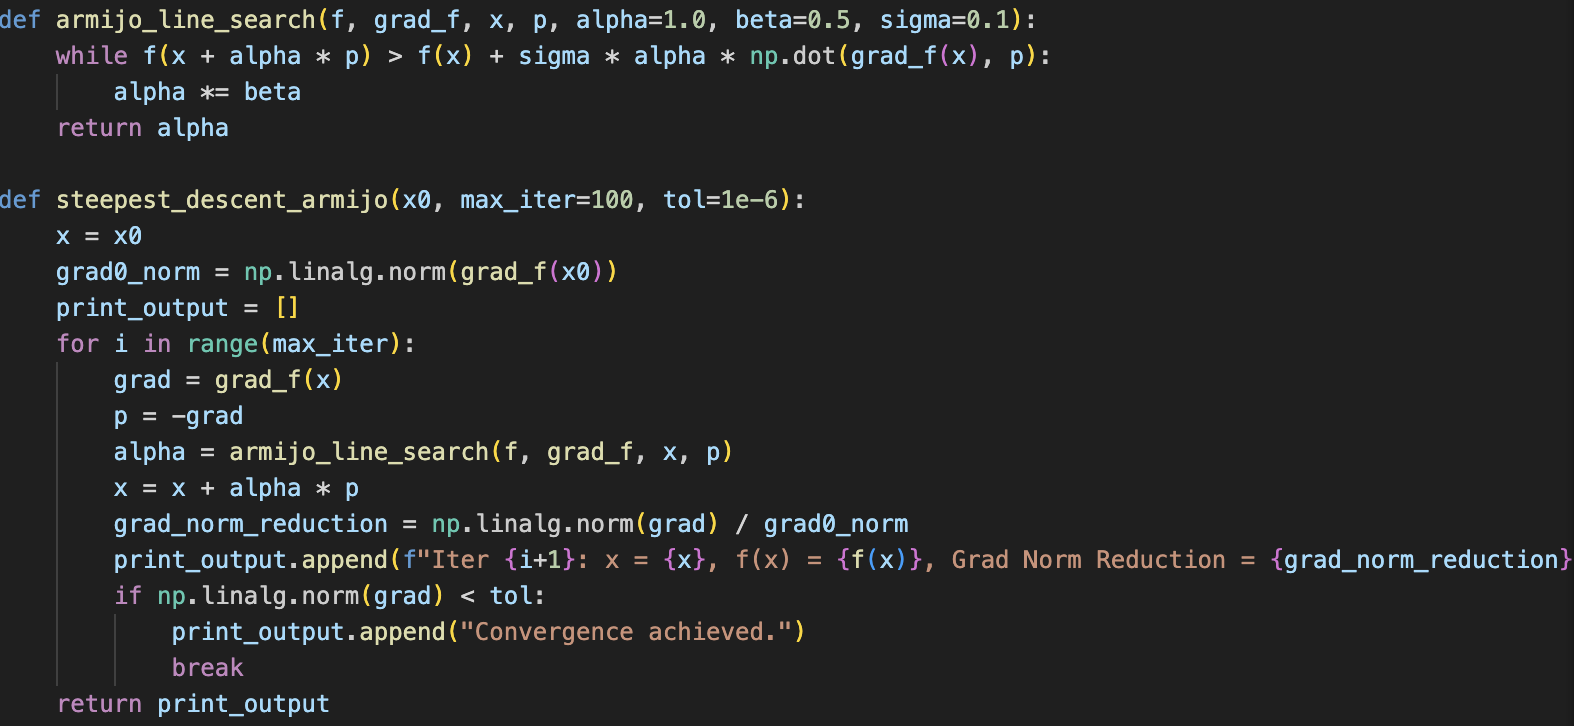
\includegraphics[width=\textwidth]{1a.png} 
    \end{figure}
    \begin{figure}[H]
    \centering
    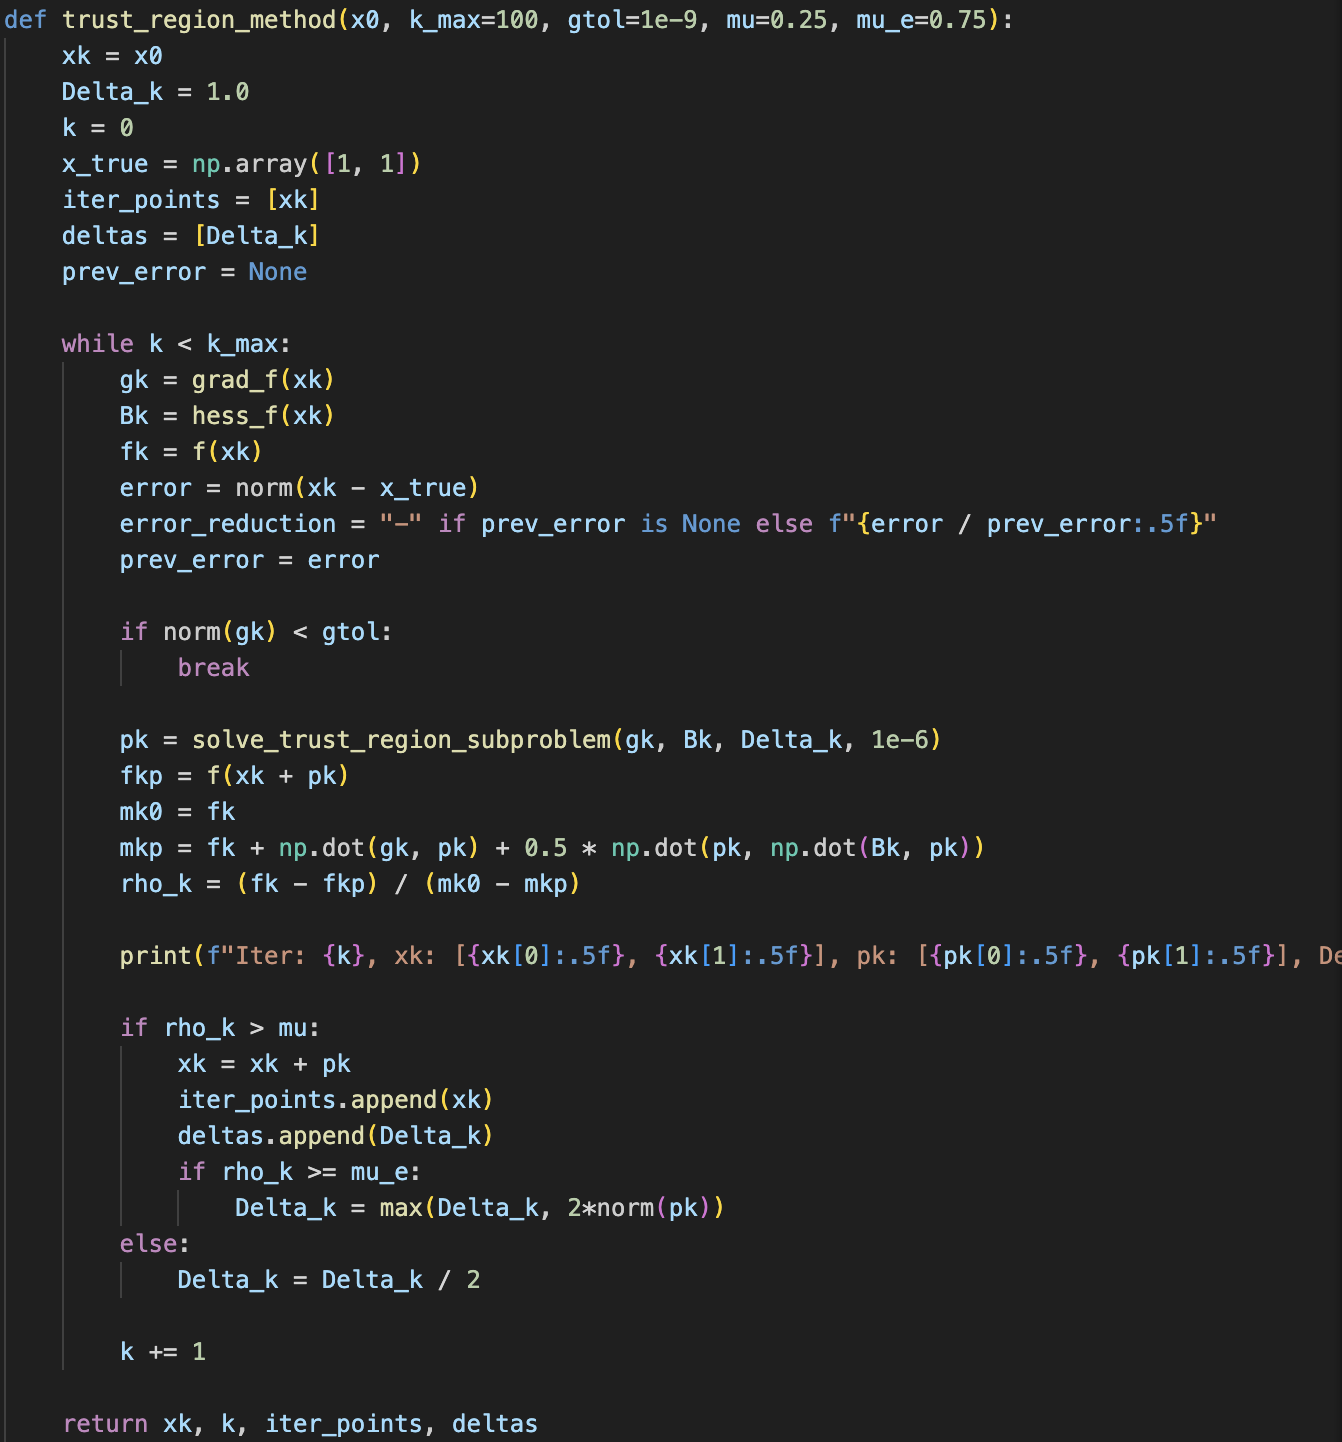
\includegraphics[width=\textwidth]{1b.png} 
    \end{figure}

    
  \item Use your implementation of the trust region method to minimize
    \textbf{Rosenbrock's function}, which in two dimensions is given by
    $$
    f(x) = (1 - x_1)^2 + 100(x_2 - x_1^2)^2.
    $$ Start with initial point $(-1,1)$. Note, the true solution for
    this problem is $x_{true} = (1, 1)$.

    \begin{figure}[H]
    \centering
    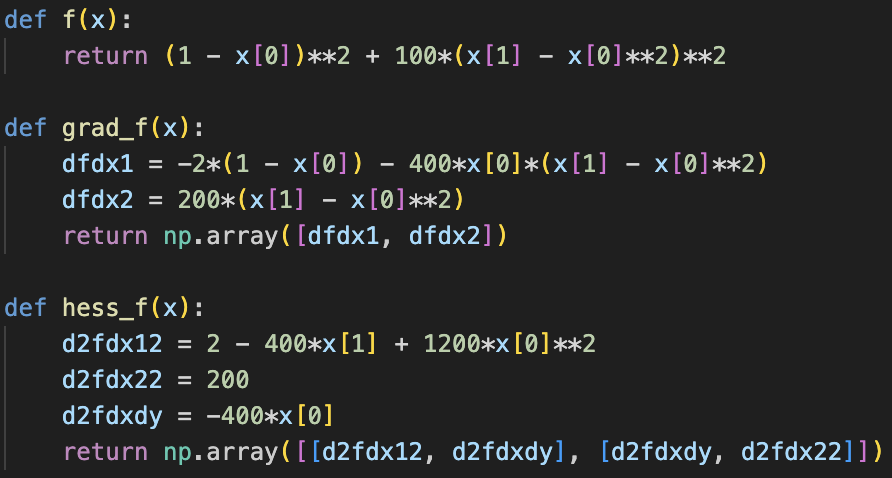
\includegraphics[width=\textwidth]{1c.png} 
    \end{figure}

    
  \item Recall the gradient and Hessian for this function.

    \begin{enumerate}
        \item[\textcolor{red}{Solution:}] 

            \textcolor{red}{The gradient is given by $\nabla f(\mathbf{x}) = \begin{pmatrix} -2(1 - x_1) - 400x_1(x_2 - x_1^2) \\ 200(x_2 - x_1^2) \end{pmatrix}$} \\
            
            \textcolor{red}{The Hessian matrix of $f$ is $\mathbf{H} = \begin{pmatrix} 2 - 400(x_2 - 3x_1^2) & -400x_1 \\ -400x_1 & 200 \end{pmatrix}$}
            
    \end{enumerate}
  
  \item Plot the objective function and the iterations on the same
    plot. {\it Hint: 2 points extracredit if you also nicely
      illustrate the trust region at every iteration.}

    \begin{figure}[H]
    \centering
    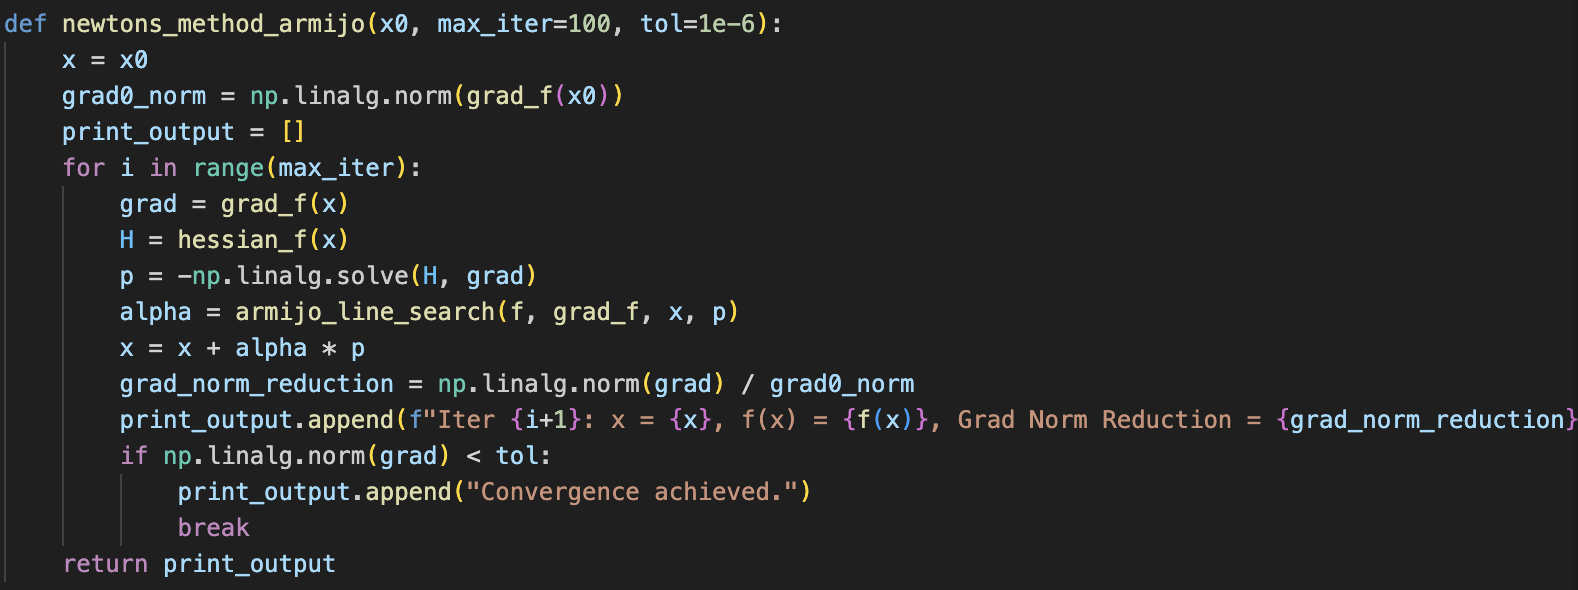
\includegraphics[width=\textwidth]{1d.png} 
    \end{figure}
      
  \item Produce a table that shows the number of iterations, the
    objective function value, the approximate solution, the norm of
    the gradient, the trust region radius, the absolute error, and the
    reduction in the error (i.e., $E_{k}/E_{k-1}$, where $E_k = ||x_k -
    x_{true}||_2$).

    \begin{figure}[H]
    \centering
    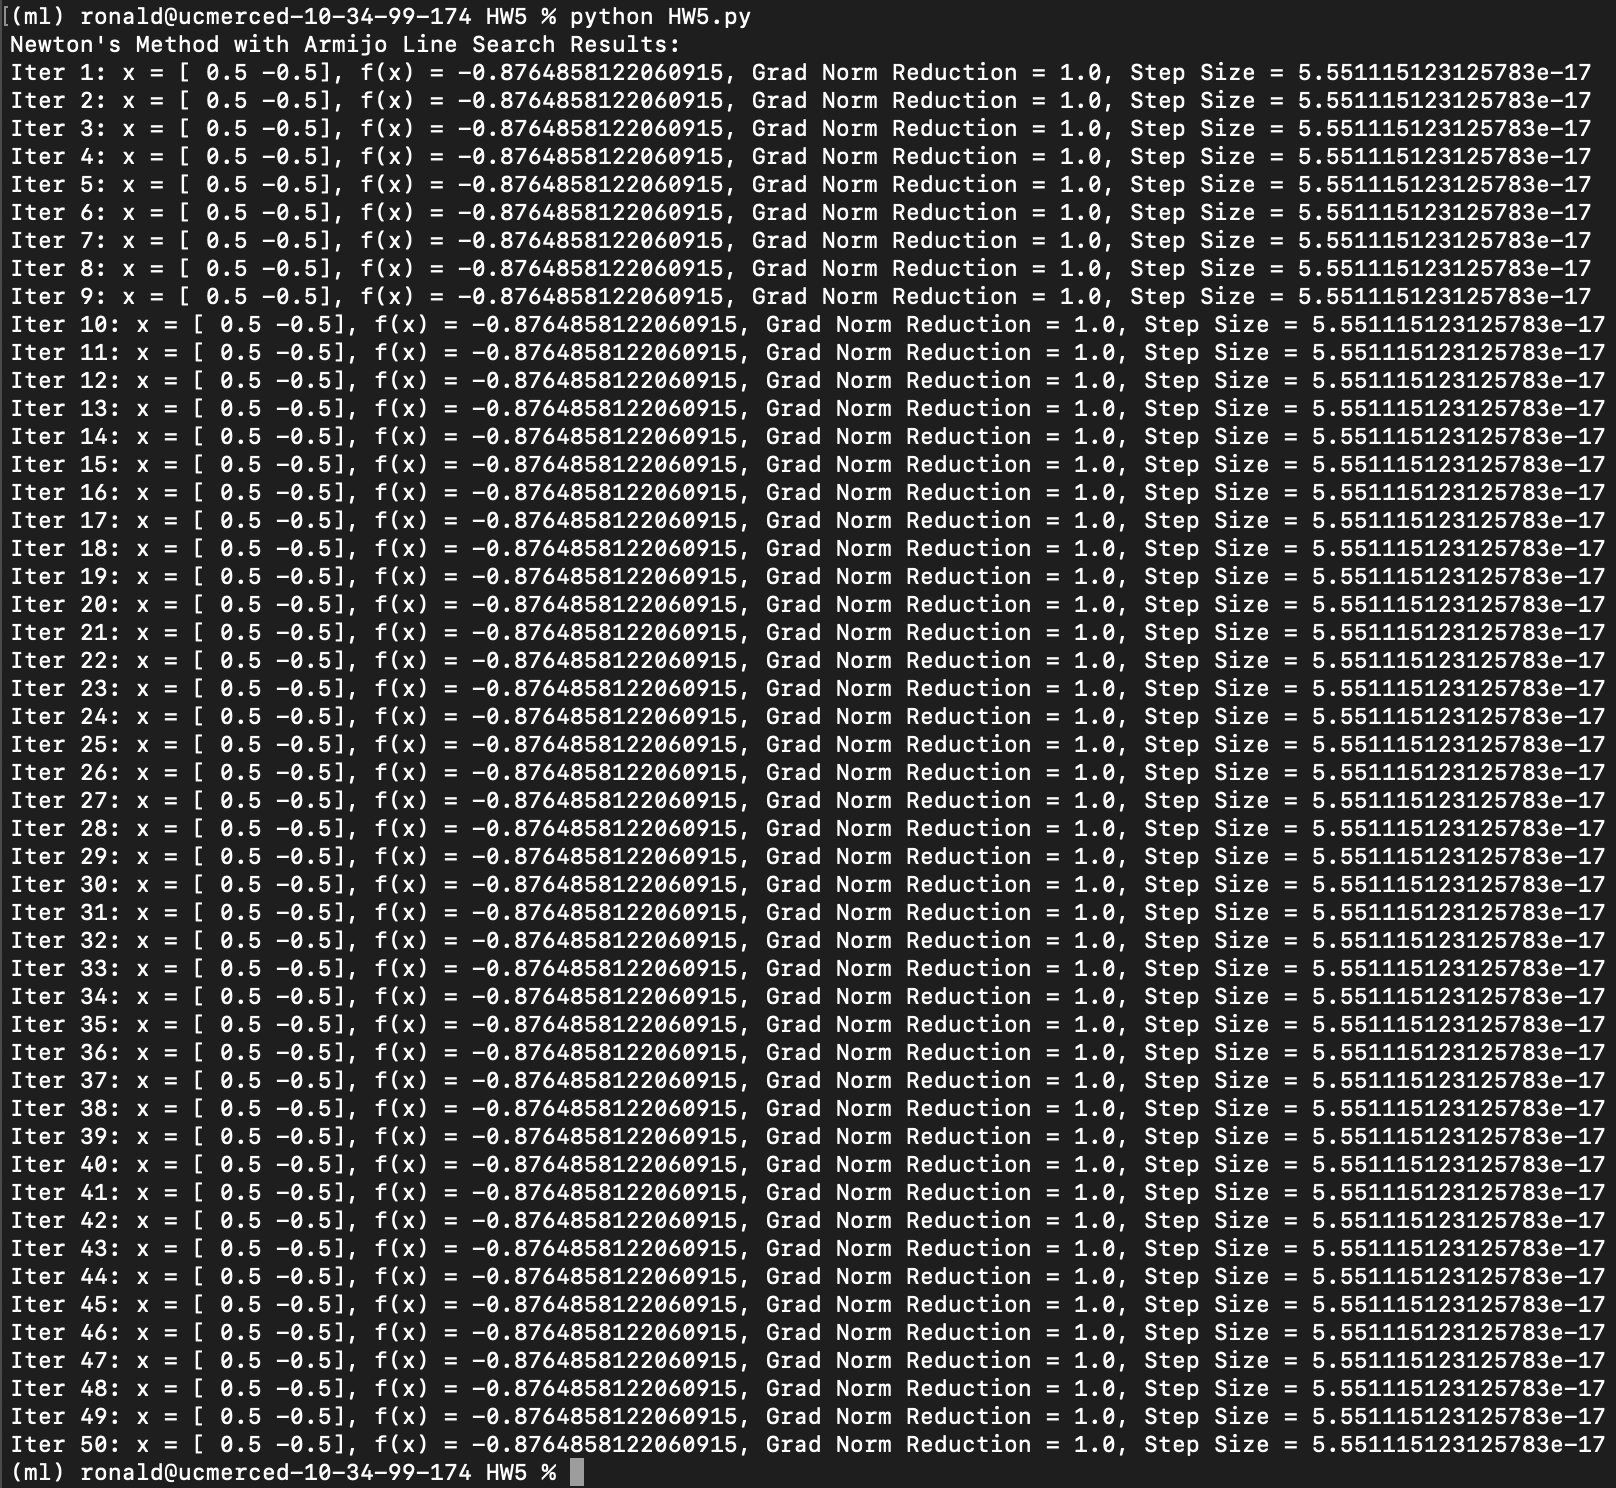
\includegraphics[width=\textwidth]{1e.png} 
    \end{figure}
    
  \item For a complete discussion of your implementation, testing, and
    results, follow the guideline on page 4. Points will be taken off
    if the required sections are missing. {\it Hint: Make sure you
      don't forget to discuss the observed convergence rate in the
      critical discussion section. Also, discuss the performance of
      the trust region method compared with line search methods, e.g.,
      steepest descent and Newton's method. No need to actually run
      your old codes but use your previous experience to compare these
      methods.}
      
    \begin{figure}[H]
    \centering
    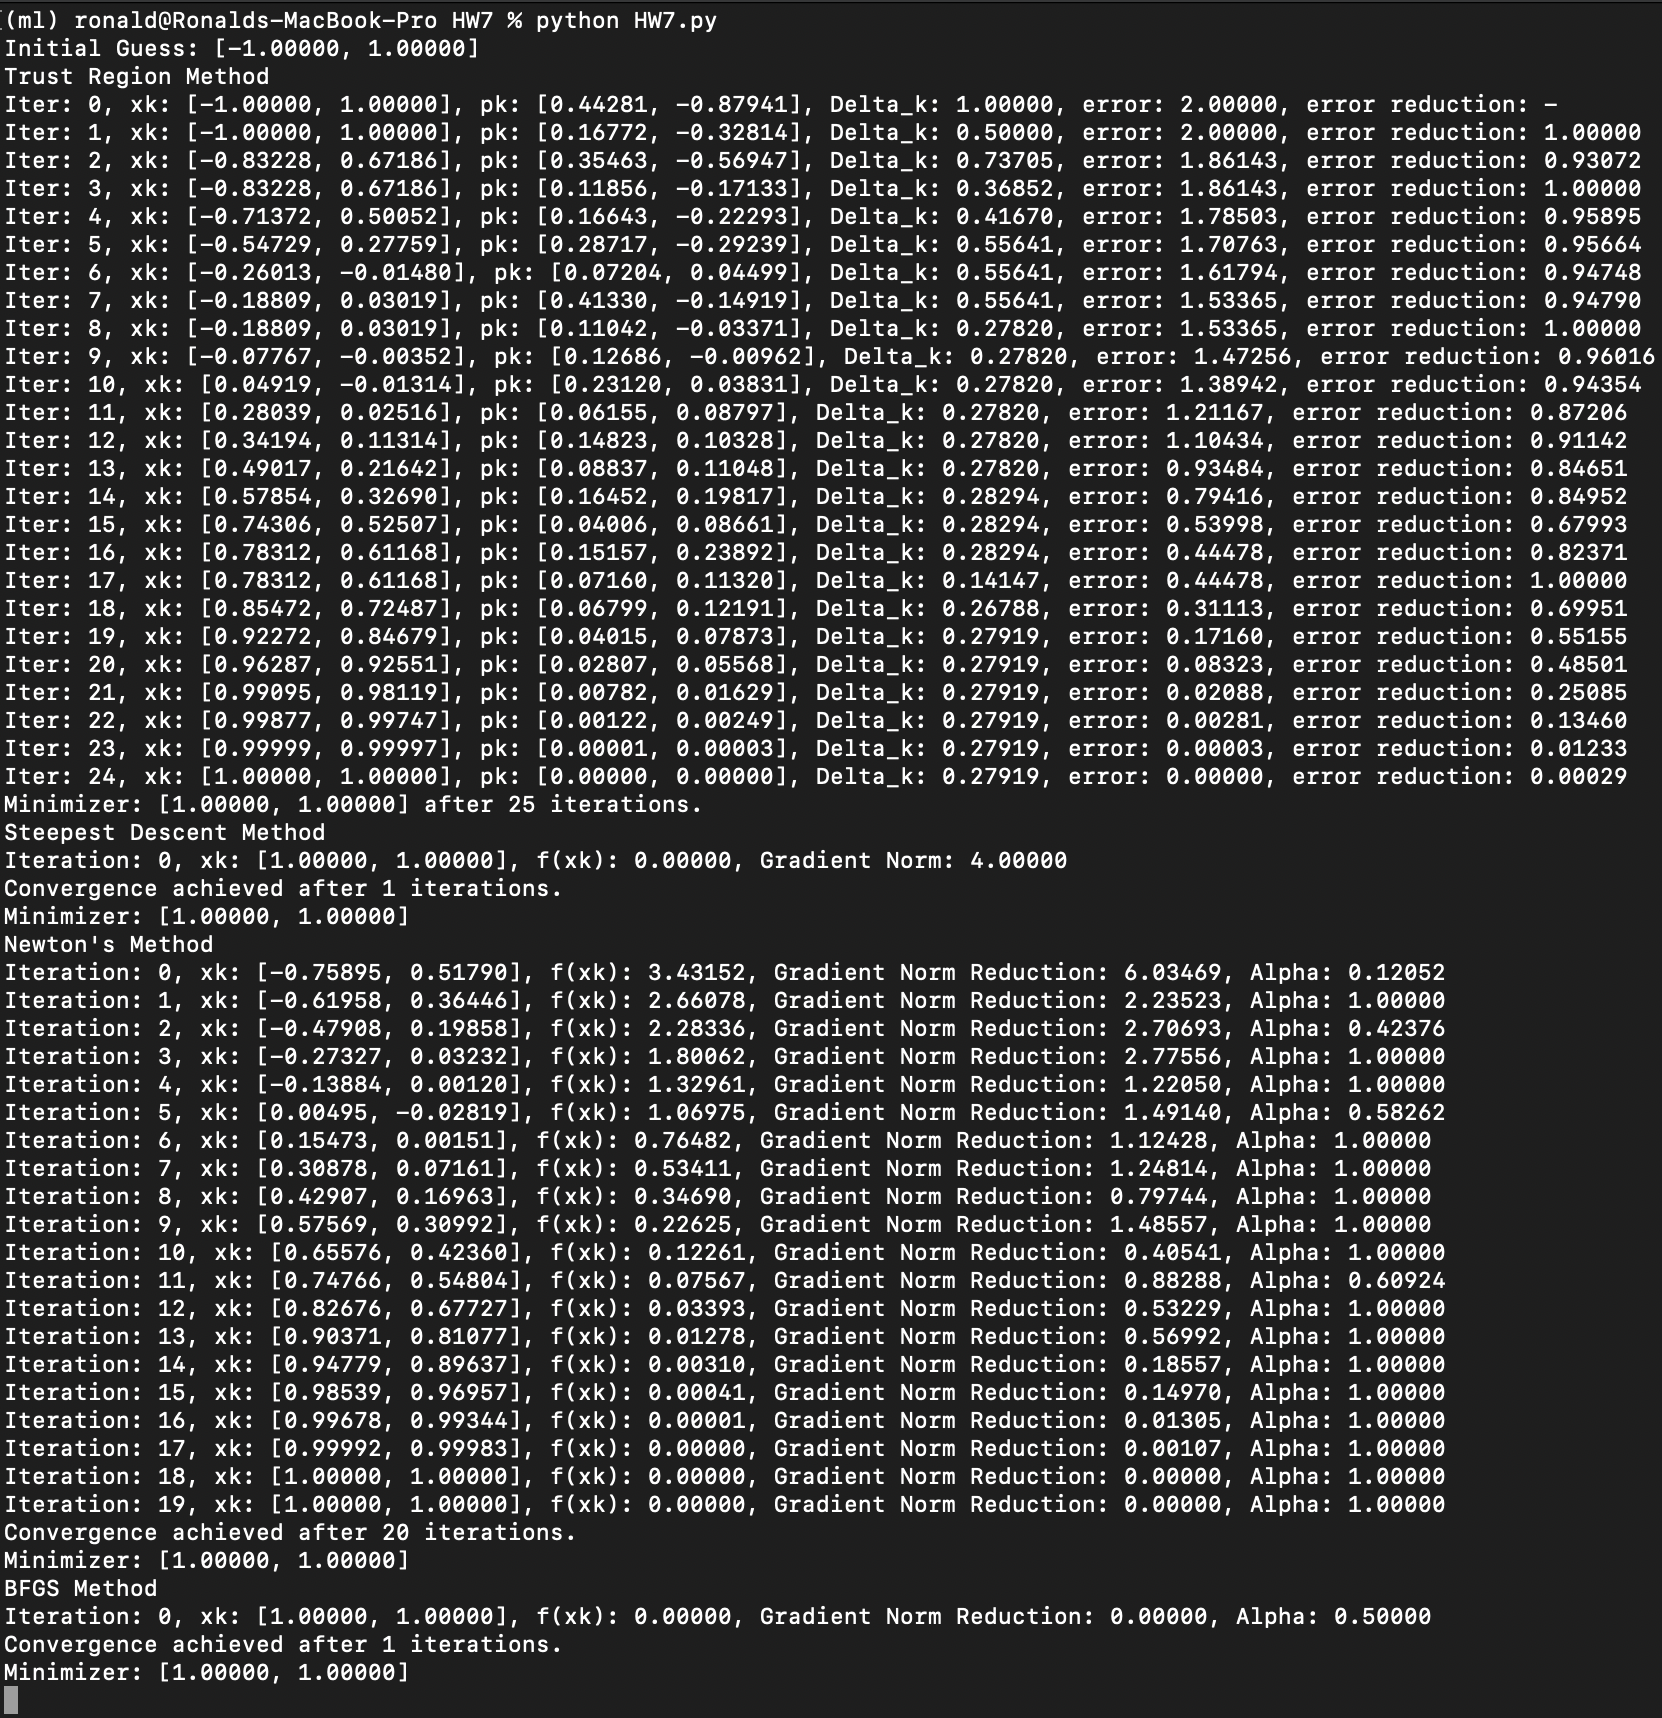
\includegraphics[width=\textwidth]{1f.png} 
    \end{figure}


    
    \item[\textcolor{red}{Solution:}] 

\textcolor{red}{To minimize Rosenbrock's function, we compare the results of different optimization techniques learned in class so far: the trust region method, the steepest descent method, and Newton's method. The trust region method leverages both the gradient and Hessian of the function to optimize within a "trust" region around the current point. The steepest descent method takes steps proportional to the negative gradient, with convergence depending on the step size in the steepest descent direction. Newton's method utilizes second-order information by involving the Hessian matrix, aiming for a quadratic convergence rate near the minimum, theoretically outpacing steepest descent. Similarly, the BFGS method approximates Newton's method without directly computing the Hessian, instead updating an estimate of its inverse at each iteration. The initial guess was set to $[-1,1]$, and the results show the trust region method converging to the known minimum $[1,1]$ in 25 iterations. Newton's method converges to $[1,1]$ in 19 iterations. Intriguingly, the steepest descent and BFGS methods indicated convergence in one iteration. However, further tests with a variety of initial guesses suggest that this swift convergence is not a feature of the algorithms themselves but rather a result of the starting point's influence. The trust region method's observed convergence aligns with theoretical expectations, converging reliably but not as swiftly as Newton's method, which is anticipated due to the latter's quadratic convergence rate.}

  \end{enumerate}
   \end{enumerate} 

  % \newpage
%\begin{eqnarray}
%	&& \underset{p \in \mathbb{R}^n}{\text{minimize }} \ \ \ m_k(p) := f_k + p^T g+ \frac{1}{2} p^T B_k p \label{eq:trustregion} \\
%	&& \text{subject to }  \ \ \| p \|_2 \le \Delta_k \nonumber
%\end{eqnarray}

%\bigskip
%\vspace{-1in}

\textbf{Algorithm 1: Trust-Region Method}

\quad Set maximum iteration $k_{\max}$, gtol, trsubtol $0 < \mu < \mu_e < 1$;

\vspace{-.15cm}

\quad $k \leftarrow 0$, $\Delta_k \leftarrow 1$, $x_k \leftarrow x_0$;

\vspace{-.15cm}

\quad \textbf{while} $k \le k_{\max}$ and $\|g_k\|_2 >= $ gtol

\vspace{-.15cm}

\quad \qquad Obtain $p_k$ by solving the TR subproblem (implement
Algorithm 2)

\vspace{-.15cm}

\quad \qquad Evaluate $\rho_k = [ f(x_k) - f(x_k+p_k) ] / [m_k(0) - m_k(p_k) ]$;

\vspace{-.15cm}

\quad \qquad \textbf{if} $\rho_k > \mu$, then

\vspace{-.15cm}

\quad \qquad \qquad $x_{k+1} = x_k + p_k$;

\vspace{-.15cm}

\quad \qquad \qquad \textbf{if} $\rho_k \ge \mu_e$ then

\vspace{-.15cm}

\quad \qquad \qquad \qquad $\Delta_{k+1} = \max \{ \Delta_k, 2\|p_k \|_2 \}$;

\vspace{-.15cm}

\quad \qquad \qquad \textbf{else}

\vspace{-.15cm}

\quad \qquad \qquad \qquad $\Delta_{k+1} = \Delta_k$;

\vspace{-.15cm}

\quad \qquad \qquad \textbf{end}

\vspace{-.15cm}

\quad \qquad \textbf{else}

\vspace{-.15cm}

\quad \qquad \qquad $x_{k+1} \leftarrow x_k$;

\vspace{-.15cm}

\quad \qquad \qquad $\Delta_{k+1} \leftarrow \frac{1}{2}\|p_k\|_2$;

\vspace{-.15cm}

\quad \qquad \textbf{end}

\vspace{-.15cm}

\quad \qquad $k \leftarrow k+1$;

\vspace{-.15cm}


\quad \textbf{end}

\bigskip


\textbf{Algorithm 2: Solving the Trust-Region Subproblem}

\quad Let $\Delta > 0$;

\vspace{-.15cm}

\quad \textbf{if} $B$ is positive definite

\vspace{-.15cm}

\quad \qquad Solve $Bp  = -g$

\vspace{-.15cm}

\quad \qquad \textbf{if} $\| p \|_2 \le \Delta$, \textbf{then} return $p$

\vspace{-.15cm}

\quad \textbf{end}

\vspace{-.15cm}

\quad Let $\lambda \ge 0$ with $B + \lambda I$ positive definite;

\vspace{-.15cm}

\quad \textbf{while} not converged

\vspace{-.15cm}

\quad \qquad Factor $B+ \lambda I = R^TR$; \quad \quad {\it Use Cholesky factorization}

\vspace{-.15cm}

\quad \qquad Solve $R^TR p = -g$;  %\quad \quad {\it First solve}

\vspace{-.15cm}

\quad \qquad Solve $R^Tu = p$;

\vspace{-.15cm}

\quad \qquad $\lambda \leftarrow \lambda +\left ( \frac{\| p \|_2}{\| u \|_2}
 	\right )^2
	\left ( 
	\frac{\| p \|_2 - \Delta}{\Delta}
	\right )
$

\quad \textbf{end}

\bigskip
Some clarifications and practical choices for the parameters present
in the TR algorithm:

\begin{enumerate}
  %\setlength{\itemsep}{0.001pt}
  \zapspace
\item Choose $B$ as the Hessian of the objective function $f(x)$.
\item For the subproblem, \verb+not converged+ means
  \begin{verbatim}
    while abs(norm(p)-Delta) > trsubtol && k < kmax,
\end{verbatim}
  where \verb+trsubtol+, \verb+k+ the current iteration, and
  \verb+kmax+ is the max number of iterations.
  \item $\mu_e = \frac{3}{4}$, $\mu = \frac{1}{4}$, gtol = $10^{-9}$,
    trsubtol = $10^{-6}$.
\end{enumerate}

% \newpage
\begin{center}
  {\bf Tips on how to report on computer results\footnote{These tips
      (with slight modifications) are from ``How to Report on Computer
      Results'' by Dr. Matthias Gobbert,
      \url{http://userpages.umbc.edu/~gobbert/teaching/math441.20158/writeup.html}}}.
      % ~\href{http://www.math.umbc.edu/~Egobbert/teaching/teaching2004to2011/math441.20098/writeup.html}{http://www.math.umbc.edu/\%7Egobbert/teaching/teaching2004to2011/math441.20098/writeup.html}}}.
\end{center}

In mathematics, as in all sciences, one of the challenges is to learn
how to communicate our findings. Therefore, I would like to guide you
to learn how to explain clearly and in a professional style what you
did and to present and analyze your results. Therefore, for this take
home exam, please follow the {\bf outline} given below for your
report. (I would recommend this outline for any homework problem that
involves computer code.)

\vspace{0.2cm}
{\bf Section 1: Problem Description}

\vspace{0.1cm} State the mathematical problem, e.g., "we want to solve
the following optimization problem ...", and state in brief words the
name of the numerical method used, e.g., "... using line search or
trust region, etc." (without stating formulas).

\vspace{0.1cm}
{\bf Section 2: Numerical Method Implemented}

\vspace{0.1cm} Explain your numerical method in detail, with suitable
formulas; you might be able to just quote a proper page of the
textbook (or recommended book), etc. This can be short if the
algorithm is stated fully somewhere (as is the case here, since the
algorithms are on page 3), but this section may be a major part of
your report, if you have to collect a lot of information from various
sources or have to derive all equations yourself. Then you should
discuss the algorithm a little, e.g., how it works, what theorems
apply, what convergence behavior you expect in which quantity, and why
you believe this might work. Here I would summarise the method as you
understood it. Give a detailed description of how you tested your
code.

{\bf Section 3: Computational Experiments and Results}

\vspace{0.1cm} Describe the computational experiments performed; that
is, state exactly the values of all parameters and other values that
have not been specified, yet. Then, introduce
your results by explaining how they are presented; you must explicitly
refer to every figure or table that you include and introduce each
function plotted or column in table. The point is to define what your
labels in the figures and tables mean. Use formulas as necessary to
define quantities clearly. You should mention results concretely,
e.g., for an error plot, you might observe that ``the absolute value of
the error is never larger than ...''.

{\bf Section 4: Critical Discussion of Results}

\vspace{0.1cm} In this section you want to contrast your results with
applicable theorems or compare results from several cases with each
other. Notice that this section is often very short, namely if you set
things up well in Section 2 (theorems quoted and convergence
expectation specified) and then plot or print out exactly these
quantities in Section 3.

{\bf References}

\vspace{0.1cm} Provide the complete bibliographic information of
your references here if and when applicable.


\end{document}

